\documentclass[10pt]{article}

\usepackage{ctex}


\usepackage{caption}
%画图
\usepackage{tikz}

%添加首行缩进,两个字符
\usepackage{indentfirst}
\setlength{\parindent}{2em}

%颜色 用法:\textcolor{name of color}{text}
\usepackage{xcolor}


%超链接
\usepackage{hyperref}
\hypersetup{
	bookmarks=true,
	colorlinks=true,
	linkcolor=black
	}


%照片
\usepackage{graphicx}

%插入python
\usepackage{pythonhighlight}

%并排放置两张图 两图的命令中间不能空行
\usepackage{subfigure}
\renewcommand{\figurename}{Figure}

%引入了一些改进的数学环境,如align
\usepackage{amsmath}

%有序列表
\usepackage{enumerate}

%插入代码
\usepackage{listings}
%插入代码的配置
\definecolor{CPPLight}  {HTML} {686868}
\definecolor{CPPSteel}  {HTML} {888888}
\definecolor{CPPDark}   {HTML} {262626}
\definecolor{CPPBlue}   {HTML} {4172A3}
\definecolor{CPPGreen}  {HTML} {487818}
\definecolor{CPPBrown}  {HTML} {A07040}
\definecolor{CPPRed}    {HTML} {AD4D3A}
\definecolor{CPPViolet} {HTML} {7040A0}
\definecolor{CPPGray}  {HTML} {B8B8B8}
\lstset{
    columns=fixed,    
    breaklines = true,   
    numbers=left,                                        % 在左侧显示行号
    frame=none,                                          % 不显示背景边框
    backgroundcolor=\color[RGB]{245,245,244},            % 设定背景颜色
    keywordstyle=\color[RGB]{40,40,255},                 % 设定关键字颜色
    numberstyle=\footnotesize\color{darkgray},           % 设定行号格式
    commentstyle=\it\color[RGB]{0,96,96},                % 设置代码注释的格式
    stringstyle=\rmfamily\slshape\color[RGB]{128,0,0},   % 设置字符串格式
    showstringspaces=false,                              % 不显示字符串中的空格
    language=Python,                                        % 设置语言
    morekeywords={True,alignas,continute,friend,register,true,alignof,decltype,goto,
    reinterpret_cast,try,asm,defult,if,return,typedef,auto,delete,inline,short,
    typeid,bool,do,int,signed,typename,break,double,long,sizeof,union,case,
    dynamic_cast,mutable,static,unsigned,catch,else,namespace,static_assert,using,
    char,enum,new,static_cast,virtual,char16_t,char32_t,explict,noexcept,struct,
    void,export,nullptr,switch,volatile,class,extern,operator,template,wchar_t,
    const,false,private,this,while,constexpr,float,protected,thread_local,
    const_cast,for,public,throw,std},
    emph={map,set,multimap,multiset,unordered_map,unordered_set,
    unordered_multiset,unordered_multimap,vector,string,list,deque,
    array,stack,forwared_list,iostream,memory,shared_ptr,unique_ptr,
    random,bitset,ostream,istream,cout,cin,endl,move,default_random_engine,
    uniform_int_distribution,iterator,algorithm,functional,bing,numeric,},
    emphstyle=\color{CPPViolet}, 
}




\title{The Fourth Week Report}
\author{Lu Guorui}
\date{2018.7.22}

%改变页边距
\usepackage[a6paper,left=10mm,right=10mm,top=15mm,bottom=15mm]{geometry}


\begin{document}

\maketitle
\renewcommand{\contentsname}{Contents}
\tableofcontents
\newpage

\addcontentsline{toc}{section}{Questions Remained}
\section*{Questions Remained}

\section{What is Forward and Back propagation?}
\indent In short, forward propagation is a way we used to count the value of compound functions. And back propagation is used to count the derivative of compound functions. We needn't complicate them.

\section{How can we express the derivative of $\sigma(z)$?}
\indent By taking the derivative of $\sigma(z)$, we can easily get the result:$\sigma'(z)=\sigma(z)(1-\sigma)$.
\indent Further, we can gain the consequence:
\begin{align}
dz = \dfrac{\partial L}{\partial z} &= \dfrac{\partial L}{\partial a}\cdot\dfrac{\partial a}{\partial z}  \\
&= (-\frac{y}{a}+\frac{1-y}{1-1}\cdot a(1-a) \\
&= a-y
\end{align}

\begin{align}
dw = \dfrac{\partial L(w,b)}{\partial w}&=\dfrac{\partial L}{\partial z}\cdot\dfrac{\partial z}{\partial w} \\
&=dz\cdot x  \\
&=x(a-y) 
\end{align}

\begin{align}
db = \dfrac{\partial L}{\partial b} &=\dfrac{\partial L}{\partial z}\cdot\dfrac{\partial z}{\partial b}  \\
&= 1\cdot dz \\
&= a-y
\end{align}

\hypersetup{
	bookmarks=true,
	colorlinks=true,
	linkcolor=red
	}


\section{Some uses of numpy. \protect\footnote{\tiny The source of package "pythonhighlight":https://github.com/chenfeng123456/python-latex-highlighting}}
\begin{enumerate}
\item Creat a vector:
\begin{python}
x = np.array([...])
\end{python}

\item Call some frequently-used functions
\begin{python}
np.exp(x)
np.log(x)
\end{python}

\item Get the shape of matrices
\begin{python}[language=Python]
x.shape[0] # the number of rows
x.shape[1] # the number of column
\end{python}

\item Change the dimension
\begin{python}
x.reshape((row,col))
\end{python}

\item Count the length of each row
\begin{python}
x_norm = np.linalg.norm(x, axis=1, keepdims = True)
\end{python}

\item Matrix-matrix or matrix-vector multiplication
\begin{python}
# matrix multiplication: 
# x1.shape = (a, m), x2.shape = (m, b)
np.dot(x1,x2) 
# multiply the elements in corresponding locations
# x1.shape = (a, m), x2.shape = (a, m)
np.multiply(x1, x2) 
\end{python}

\item Gain random numbers

\begin{itemize}

\item Get one number
\begin{python}
n = numpy.random.random()
\end{python}

\item Get a matrix
\begin{python}
n = numpy.random.random(size=(3, 2))
\end{python}

\item Generate random numbers between 0 and 1
\begin{python}
np.random.rand(2,3) # (2,3) show the dimension
\end{python}

\item Generate the same random numbers
\begin{python}
'''
Set the same seed every time,
and we can get the same random numbers
'''
numpy.random.seed(num)
numpy.random.rand(the_length_of_array)
\end{python}

\end{itemize}


\end{enumerate} 

\section{What do high bias and high variance mean?}
\indent High bias means that your model can't fit your train set well and high variance means your model overfit the train set so that it can't fit other data well.

\begin{figure}[htbp]

\begin{minipage}[t]{0.45\linewidth}
\centering
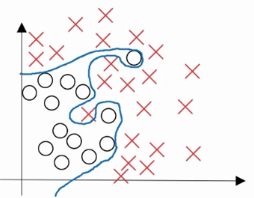
\includegraphics[width=3cm]{overfit.png}
\caption{Overfitting}
\label{overfitting}
\end{minipage}
\hfill %中间不能空行
\begin{minipage}[t]{0.45\linewidth}
\centering
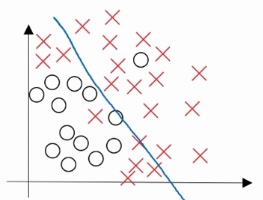
\includegraphics[width=3cm]{underfitting.png}
\caption{Underfitting}
\label{underfitting}
\end{minipage}
\end{figure}



\section{\protect\textcolor{red}{How does regularization prevent overfitting?}}
\indent Regularization is able to reduce overfitting by adding the regularization term, $\dfrac{\lambda}{2m}||w||_{2}^{2}$. So the derivative $\dfrac{\partial L}{\partial W}$ turns into: $dW^{[l]}=(form\_backprop)+\dfrac{\lambda}{m}W^{[l]}$. Then we can get the update of grads as follows:
\begin{align}
W^{[l]}:&=W^{[l]}-\alpha [ (form\_backprop)+\dfrac{\lambda}{m}W^{[l]}]\\
&=W^{[l]}-\alpha\dfrac{\lambda}{m}W^{[l]}-\alpha(form\_backprop)\\
&=(1-\dfrac{\alpha\lambda}{m})W^{[l]}-\alpha(form\_backprop)
\end{align} 




\indent If $\lambda$ is big enough, the weight matrix $W$ can be very small, and so does the $Z$. As the \autoref{tanh} shows, when $Z$ is relatively small, $tanh(Z)$ could be almost linear. We have known that when $g(x)$ is linear, no matter how deep the neural network is, what it counts is alaways a linear function which can't fit very complicate data.

\indent Of course we need't keep $Z$ so small all the time, but we can find a reasonable range that makes our model "just right".

\par
\begin{figure}[htbp]
\begin{tikzpicture}[yscale=1.5]
\draw [help lines, <->] (-4,0) -- (4,0);
\draw [help lines, ->] (0,-1.1) -- (0,1.1);
\draw [blue,domain=-4:4] plot (\x,{tanh(\x)});
\draw[fill] (0.5,{tanh(0.5)}) circle [radius=0.025];
\node [below right, red] at (0.5,{tanh(0.5)}){$A$};
\draw[fill] (-0.5,{tanh(-0.5)}) circle [radius=0.025];
\node [above left, red] at (-0.5,{tanh(-0.5)}){$B$};
\node [right, black] at (4,0){$Z$};
\node [above, black] at (0,1.1){$tanh(Z)$};
\end{tikzpicture}
\caption{$tanh(Z)$ function}
\label{tanh}%label 必须放在caption后面
\end{figure}



\end{document}